%%%%%%%%%%%%%%%%%%%%%%%%%%
%%  Capítulo 2: Fundamentos de antenas de abertura  %%
%%%%%%%%%%%%%%%%%%%%%%%%%%

%%%%
\section{Integrales de radiación y potenciales vectoriales}
\label{sec_fundamentos_integrales}
%%%%

%%%%
Las ecuaciones de Maxwell con fuentes, considerando campos armónicos, se expresan como:
%%%%
\begin{align}
\divergencia{D} &= \rho_e
\label{ec_fundamentos:1}\\
\divergencia{B} &= 0
\label{ec_fundamentos:2}\\
\rotor{E} &= - j\omega\mathbf{B}
\label{ec_fundamentos:3}\\
\rotor{H} &= \mathbf{J} + j\omega\mathbf{D}
\label{ec_fundamentos:4}
\end{align}
%%%%
Para facilitar la resolución de estas ecuaciones inhomogéneas, se definen funciones auxiliares denominadas \emph{potenciales vectoriales y escalares}. Los potenciales vectoriales más comunes son el potencial vectorial magnético $\mathbf{A}$ y el potencial vectorial eléctrico $\mathbf{F}$ \cite{Balanisantenas}.

El potencial vectorial $\mathbf{A}$ se utiliza para determinar los campos generados por una densidad de corriente $\mathbf{J}$. Según la ecuación \eqref{ec_fundamentos:2}, la divergencia del flujo magnético $\mathbf{B}$ es cero, es decir, el campo magnético es selenoidal, razón por la que $\mathbf{B}$ puede reemplazarse por el rotor de otro vector, ya que responde a la identidad vectorial:
%%%%
\begin{align}
\divergencia{B} = \divergencia{}\rotor{A} = 0
\label{ec_fundamentos:5}
\end{align}
%%%%
donde $\mathbf{A}$ es el potencial vectorial magnético. Se define entonces:
%%%%
\begin{align}
\mathbf{H}_A = \frac{1}{\mu}\rotor{A}
\label{ec_fundamentos:6}
\end{align}
%%%%
Reemplazando en la ecuación de Maxwell \eqref{ec_fundamentos:3}, se obtiene:
%%%%
\begin{align}
\rotor{}\left(\mathbf{E}_A + j\omega\mathbf{A}\right) = 0
\label{ec_fundamentos:7}
\end{align}
%%%%
Se emplea la identidad vectorial:
%%%%
\begin{align}
\rotor{}\left(- \gradiente\phi_e\right) = 0
\label{ec_fundamentos:8}
\end{align}
%%%%
donde $\phi_e$ se denomina \emph{potencial escalar eléctrico}. A partir de las expresiones \eqref{ec_fundamentos:7} y \eqref{ec_fundamentos:8}, se llega a:
%%%%
\begin{align}
\mathbf{E}_A = - \gradiente\phi_e - j\omega\mathbf{A}
\label{ec_fundamentos:9}
\end{align}
%%%%
Aplicando el rotor a ambos lados de la expresión \eqref{ec_fundamentos:6} y utilizando la siguiente identidad vectorial:
%%%%
\begin{align}
\rotor{}\rotor{A} = \gradiente\left(\divergencia{A}\right) - \laplaciano{A}
\label{ec_fundamentos:10}
\end{align}
%%%%
se obtiene:
%%%%
\begin{align}
\mu\rotor{H}_A = \gradiente\left(\divergencia{A}\right) - \laplaciano{A}
\label{ec_fundamentos:11}
\end{align}
%%%%
Empleando la ecuación de Maxwell \eqref{ec_fundamentos:4}, la expresión \eqref{ec_fundamentos:11} resulta:
%%%%
\begin{align}
\mu\mathbf{J} + j\omega\mu\varepsilon\mathbf{E}_A = \gradiente\left(\divergencia{A}\right) - \laplaciano{A}
\label{ec_fundamentos:12}
\end{align}
%%%%
y utilizando la expresión \eqref{ec_fundamentos:9}, se obtiene:
%%%%
\begin{align}
\laplaciano{A} + \omega^2\mu\varepsilon\mathbf{A} = - \mu\mathbf{J} + \gradiente\left(\divergencia{A} + j\omega\mu\varepsilon\phi_e\right)
\label{ec_fundamentos:13}
\end{align}
%%%%
Todo campo vectorial queda unívocamente definido si se conoce su rotor y su divergencia. El rotor del potencial vectorial $\mathbf{A}$ fue definido en la expresión \eqref{ec_fundamentos:6}, pero las ecuaciones de Maxwell no dan ninguna condición sobre su divergencia, por lo que puede elegirse de la forma más conveniente para resolver el problema. Para tal fin, se utiliza la \emph{calibración de Lorentz}, que se define como:
%%%%
\begin{align}
\divergencia{A} = - j\omega\mu\varepsilon\phi_e \Longrightarrow \phi_e = - \frac{1}{j\omega\mu\varepsilon}\divergencia{A}
\label{ec_fundamentos:14}
\end{align}
%%%%
Con la calibración de Lorentz, la expresión \eqref{ec_fundamentos:9} resulta:
%%%%
\begin{align}
\mathbf{E}_A = - j\omega\mathbf{A} - j\frac{1}{\omega\mu\varepsilon}\gradiente\left(\divergencia{A}\right)
\label{ec_fundamentos:15}
\end{align}
%%%%
mientras que la expresión \eqref{ec_fundamentos:13} se reduce a:
%%%%
\begin{align}
\laplaciano{A} + \omega^2\mu\varepsilon\mathbf{A} = - \mu\mathbf{J}
\label{ec_fundamentos:16}
\end{align}
%%%%
que corresponde a una ecuación de ondas vectorial inhomogénea, cuya solución es el potencial vectorial $\mathbf{A}$.

Las corrientes magnéticas no existen físicamente, pero se emplean como una herramienta auxiliar al aplicar teoremas de equivalencia de volúmenes o de superficie. Mediante el teorema de dualidad electromagnética, es posible expresar la solución de un problema con una fuente magnética a partir de la solución para un problema similar con una fuente eléctrica.

Las ecuaciones de Maxwell, aplicando el teorema de dualidad \cite{Balanisantenas}, quedan expresadas como:
%%%%
\begin{align}
\divergencia{B} &= \rho_m
\label{ec_fundamentos:17}\\
\divergencia{D} &= 0
\label{ec_fundamentos:18}\\
\rotor{H} &= j\omega\mathbf{D}
\label{ec_fundamentos:19}\\
\rotor{E} &= - \mathbf{M} - j\omega\mathbf{B}
\label{ec_fundamentos:20}
\end{align}
%%%%
Los campos debidos al potencial vectorial $\mathbf{F}$ resultan:
%%%%
\begin{align}
\mathbf{E}_F &= - \frac{1}{\varepsilon}\rotor{F}
\label{ec_fundamentos:21}\\
\mathbf{H}_F &= - j\omega\mathbf{F} - j\frac{1}{\omega\mu\varepsilon}\gradiente\left(\divergencia{F}\right)
\label{ec_fundamentos:22}
\end{align}
%%%%
donde el potencial vectorial $\mathbf{F}$ es la solución de la ecuación de ondas vectorial inhomogénea:
%%%%
\begin{align}
\laplaciano{F} + \omega^2\mu\varepsilon\mathbf{F} = - \varepsilon\mathbf{M}
\label{ec_fundamentos:23}
\end{align}
%%%%
En resumen, el procedimiento que puede ser usado para hallar los campos es el siguiente:
%%%%
\begin{enumerate}
\item Especificar las densidades de corriente eléctrica $\mathbf{J}$ y magnética $\mathbf{M}$.
\item Hallar el potencial vectorial $\mathbf{A}$ usando:
%%%%
\begin{align}
\mathbf{A} = \frac{\mu}{4\pi}\iiint\limits_V\mathbf{J}\frac{e^{-jkR}}{R}\,dv'
\label{ec_fundamentos:24}
\end{align}
%%%%
que es la solución de la ecuación de ondas vectorial inhomogénea \eqref{ec_fundamentos:16}.
\item Hallar el potencial vectorial $\mathbf{F}$ usando:
%%%%
\begin{align}
\mathbf{F} = \frac{\varepsilon}{4\pi}\iiint\limits_V\mathbf{M}\frac{e^{-jkR}}{R}\,dv'
\label{ec_fundamentos:25}
\end{align}
%%%%
que es la solución de la ecuación de ondas vectorial inhomogénea \eqref{ec_fundamentos:23}. En las expresiones \eqref{ec_fundamentos:24} y \eqref{ec_fundamentos:25}, $k^2 = \omega^2\mu\varepsilon$ y $R$ es la distancia entre un punto de la fuente y el punto de observación.
\item Hallar los campos debidos al potencial vectorial $\mathbf{A}$.
\item Hallar los campos debidos al potencial vectorial $\mathbf{F}$.
\item El campo total $\mathbf{E}$ está determinado por:
%%%%
\begin{align}
\mathbf{E} = \mathbf{E}_A + \mathbf{E}_F = - jw\mathbf{A} - j\frac{1}{\omega\mu\varepsilon}\gradiente\left(\divergencia{A}\right) - \frac{1}{\varepsilon}\rotor{F}
\label{ec_fundamentos:26}
\end{align}
%%%%
\item El campo total $\mathbf{H}$ está determinado por:
%%%%
\begin{align}
\mathbf{H} = \mathbf{H}_A + \mathbf{H}_F = - jw\mathbf{F} - j\frac{1}{\omega\mu\varepsilon}\gradiente\left(\divergencia{F}\right) + \frac{1}{\mu}\rotor{A}
\label{ec_fundamentos:27}
\end{align}
%%%%
\end{enumerate}
%%%%

%%%%
\section{Principio de equivalencias de campos}
\label{sec_fundamentos_principio}
%%%%

%%%%
La \emph{equivalencia de campos} es un principio por el cual las fuentes de radiación reales son reemplazadas por fuentes equivalentes.
%%%%
\begin{figure} [H]
\centering 
\subfigure[Problema real.]{
\label{fig_fundamentos:1}
\raisebox{0.3312cm}{
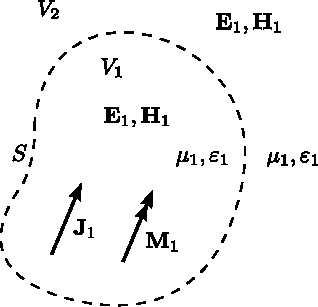
\includegraphics[scale = 1]{Figures/Fundamentos/fundamentos_1.pdf}}}
\hspace{0.5cm}
\subfigure[Problema equivalente.]{
\label{fig_fundamentos:2}
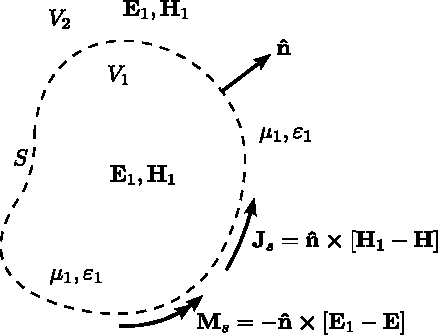
\includegraphics[scale = 1]{Figures/Fundamentos/fundamentos_2.pdf}}
\caption{Modelos real y equivalente del principio de equivalencia de campos.}
\label{grup_fig_fundamentos:1}
\end{figure}
%%%%
Toda fuente de radiación puede representarse eléctricamente por las densidades de corriente eléctrica $\mathbf{J}$ y magnética $\mathbf{M}$. Como se muestra en la figura \ref{fig_fundamentos:1}, las fuentes $\mathbf{J}_1$ y $\mathbf{M}_1$ están encerradas en una superficie $S$ e irradian los campos $\mathbf{E}_1$ y $\mathbf{H}_1$ en todas las direcciones. El volumen dentro de $S$ se denota mediante $V_1$, y fuera de $S$ mediante $V_2$. El objetivo principal es reemplazar el problema original, que se muestra en la figura \ref{fig_fundamentos:1}, por uno equivalente de la figura \ref{fig_fundamentos:2} que produzca los mismos campos $\mathbf{E}_1$ y $\mathbf{H}_1$ fuera de $S$ (dentro de $V_2$). Para que estos campos existan fuera de $S$, se deberán satisfacer las condiciones de contorno de las componentes tangenciales de los campos eléctrico y magnético. De esta forma, sobre la superficie imaginaria $S$ deben existir las fuentes equivalentes, cuyas expresiones son:
%%%%
\begin{align}
\mathbf{J}_s &= \versor{n}\prodvec\left[\mathbf{H}_1 - \mathbf{H}\right]
\label{ec_fundamentos:28}\\
\mathbf{M}_s &= - \versor{n}\prodvec\left[\mathbf{E}_1 - \mathbf{E}\right]
\label{ec_fundamentos:29}
\end{align}
%%%%
Como los campos dentro de $S$ pueden tener cualquier valor, por conveniencia se consideran nulos. En ese caso, el problema equivalente de la figura \ref{fig_fundamentos:2} se reduce al de la figura \ref{fig_fundamentos:3}, con las densidades de corriente equivalentes siendo iguales a:
%%%%
\begin{align}
\mathbf{J}_s &= \versor{n}\prodvec\left.\left[\mathbf{H}_1 - \mathbf{H}\right]\right|_{\mathbf{H} = 0} \Longrightarrow \mathbf{J}_s = \versor{n}\prodvec\mathbf{H}_1
\label{ec_fundamentos:30}\\
\mathbf{M}_s &= - \versor{n}\prodvec\left.\left[\mathbf{E}_1 - \mathbf{E}\right]\right|_{\mathbf{E} = 0} \Longrightarrow \mathbf{M}_s = - \versor{n}\prodvec\mathbf{E}_1
\label{ec_fundamentos:31}
\end{align}
%%%%
Esta forma del principio de equivalencia de campos es conocida como \emph{Principio de equivalencia de Love}.
%%%%
\begin{figure} [H]
\centering 
\subfigure[Equivalente de Love.]{
\label{fig_fundamentos:3}
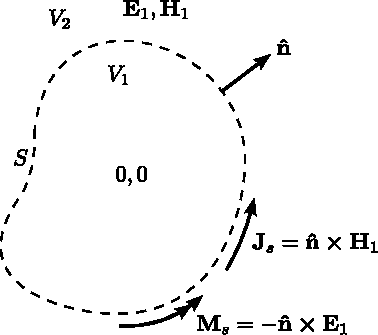
\includegraphics[scale = 1]{Figures/Fundamentos/fundamentos_3.pdf}}
\hspace{0.5cm}
\subfigure[Equivalente para conductor eléctrico.]{
\label{fig_fundamentos:4}
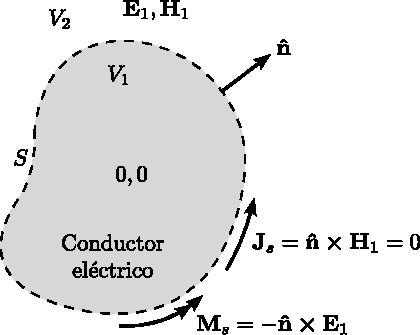
\includegraphics[scale = 1]{Figures/Fundamentos/fundamentos_4.pdf}}
\caption{Modelos del principio de equivalencia.}
\label{grup_fig_fundamentos:2}
\end{figure}
%%%%
Aunque el medio interior se modifique, $\mathbf{E}$ y $\mathbf{H}$ continuarán siendo nulos.  Si el medio interior es reemplazado por un conductor eléctrico perfecto, la densidad de corriente eléctrica $\mathbf{J}_s$, que es tangencial a la superficie $S$, es cortocircuitada por el conductor eléctrico; de esta forma, el problema equivalente de la figura \ref{fig_fundamentos:3} se reduce al de la figura \ref{fig_fundamentos:4}.

Para encontrar la utilidad al principio de equivalencia de campos, especialmente para el problema de la figura \ref{fig_fundamentos:4}, se asume que la superficie $S$ es un conductor eléctrico plano y que se extiende hasta el infinito, como se muestra en la figura \ref{fig_fundamentos:5}. Para esta geometría, el problema radica en cómo una fuente magnética irradia en presencia de un conductor eléctrico plano, por lo que aplicando teoría de imágenes se reduce el problema al de la figura \ref{fig_fundamentos:6}. Como la fuente imaginaria está en la misma dirección que la fuente equivalente, el problema equivalente de la figura \ref{fig_fundamentos:6} se reduce al de la figura \ref{fig_fundamentos:7}.
%%%%
\begin{figure} [H]
\centering 
\subfigure[]{
\label{fig_fundamentos:5}
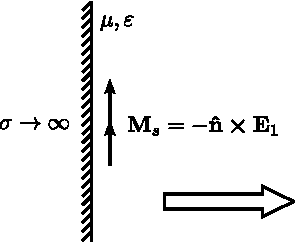
\includegraphics[scale = 1]{Figures/Fundamentos/fundamentos_5.pdf}}
\subfigure[]{
\label{fig_fundamentos:6}
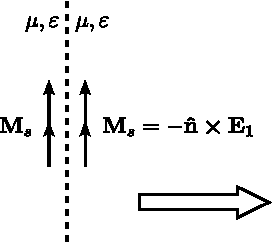
\includegraphics[scale = 1]{Figures/Fundamentos/fundamentos_6.pdf}}
\subfigure[]{
\label{fig_fundamentos:7}
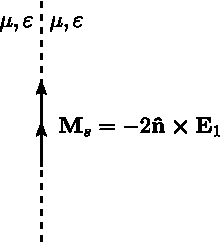
\includegraphics[scale = 1]{Figures/Fundamentos/fundamentos_7.pdf}}
\caption{Modelos equivalentes para fuentes magnéticas cercanas a un conductor eléctrico perfecto.}
\label{grup_fig_fundamentos:3}
\end{figure}
%%%%
Considerando una abertura montada sobre un plano conductor infinito y conociendo los campos $\mathbf{E}_a$ y $\mathbf{H}_a$ sobre dicha abertura, es posible determinar las densidades de corriente $\mathbf{M}_s$ y $\mathbf{J}_s$ resolviendo el problema análogamente al de la figura \ref{grup_fig_fundamentos:3}. El resultado puede verse en la figura \ref{grup_fig_fundamentos:4}: mientras que en la figura \ref{fig_fundamentos:8} la abertura es excitada con campo distribuido uniformemente, en la figura \ref{fig_fundamentos:9} se emplea una guía de ondas, por lo que la excitación se produce mediante campo con distribución sinusoidal.
%%%%
\begin{figure} [H]
\centering 
\subfigure[Excitación con campo distribuido uniformemente.]{
\label{fig_fundamentos:8}
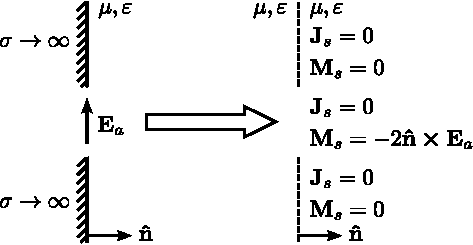
\includegraphics[scale = 1]{Figures/Fundamentos/fundamentos_8.pdf}}
\subfigure[Excitación con campo con distribución sinusoidal.]{
\label{fig_fundamentos:9}
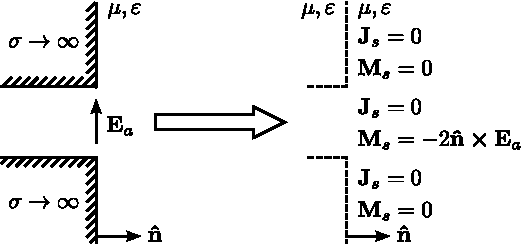
\includegraphics[scale = 1]{Figures/Fundamentos/fundamentos_9.pdf}}
\caption{Modelos equivalentes empleados para aberturas montadas sobre un plano conductor infinito.}
\label{grup_fig_fundamentos:4}
\end{figure}
%%%%
Las guías de onda con extremo abierto y bocinas no están montadas sobre un plano conductor infinito, lo que implica que la densidad de corriente $\mathbf{J}_s$ sobre la abertura no es cortocircuitada y, por lo tanto, no es nula. El problema es que a priori los campos fuera de la abertura no son conocidos, por lo que a pesar de existir un equivalente exacto del problema, no puede utilizarse. Lo más ususal es asumir que $\mathbf{E}_a$ y $\mathbf{H}_a$ (y por lo tanto, $\mathbf{M}_s$ y $\mathbf{J}_s$), existen sobre la abertura pero son nulos fuera de ella, como puede observarse en la figura \ref{fig_fundamentos:10}. Se ha demostrado, mediante comparación con mediciones y otros datos disponibles, que este modelo equivalente aproximado es el que mejores resultados produce \cite{Balanisantenas}.
%%%%
\begin{figure} [H]
\centering 
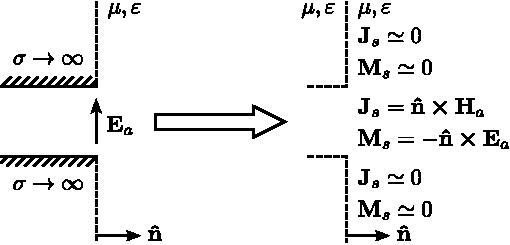
\includegraphics[scale = 1]{Figures/Fundamentos/fundamentos_10.pdf}
\caption{Modelo equivalente empleado para guías de onda con extremo abierto y bocinas.}
\label{fig_fundamentos:10}
\end{figure}
%%%%
Puede deducirse, a partir de las expresiones de las densidades de corriente $\mathbf{J}_s$ y $\mathbf{M}_s$ de los modelos empleados para las distintas antenas de abertura, que solamente las componentes tangenciales de los campos $\mathbf{E}_a$ y $\mathbf{H}_a$ son las responsables de la radiación.

Para el modelo equivalente de la figura \ref{fig_fundamentos:10}, $\mathbf{H}_a$ y $\mathbf{E}_a$ están relacionados entre sí mediante la expresión:
%%%%
\begin{align}
&\mathbf{H}_a = \versor{n}\prodvec\frac{\mathbf{E}_a}{\eta}
\label{ec_fundamentos:32}
\end{align}
%%%%

%%%%
\section{Campos radiados}
\label{sec_fundamentos_campos}
%%%%

%%%%
Para observaciones de campo lejano, la componente radial de los campos radiados es despreciable, por lo que se considera que $\mathbf{E}$ y $\mathbf{H}$ tienen solamente componentes en los ángulos $\uptheta$ y $\upphi$; a la vez el frente de onda, que es esférico, puede aproximarse a un frente de onda plano, por lo que los campos $\mathbf{E}$ y $\mathbf{H}$ están relacionados entre sí mediante la impedancia intrínseca del medio. Partiendo de las expresiones \eqref{ec_fundamentos:26} y \eqref{ec_fundamentos:27} y despreciando las componentes radiales, los campos $\mathbf{E}$ y $\mathbf{H}$ pueden expresarse como:
%%%%
\begin{align}
\mathbf{E} &\simeq - jw\mathbf{A} + j\omega\eta\left(\versor{r}\prodvec\mathbf{F}\right)
\label{ec_fundamentos:33}\\
\mathbf{H} &\simeq \versor{r}\prodvec\frac{\mathbf{E}}{\eta}
\label{ec_fundamentos:34}
\end{align}
%%%%
y las componentes de ambos campos como:
%%%%
\begin{subequations}
\label{grup_ec_fundamentos:1}
\begin{align}
E_r &\simeq 0
\label{ec_fundamentos:35}\\
E_{\theta} &\simeq - j\omega\left(A_{\theta} + \eta F_{\phi}\right)
\label{ec_fundamentos:36}\\
E_{\phi} &\simeq - j\omega\left(A_{\phi} - \eta F_{\theta}\right)
\label{ec_fundamentos:37}\\
H_r &\simeq 0
\label{ec_fundamentos:38}\\
H_{\theta} &\simeq - \frac{E_{\phi}}{\eta}
\label{ec_fundamentos:39}\\
H_{\phi} &\simeq \frac{E_{\theta}}{\eta}
\label{ec_fundamentos:40}
\end{align}
\end{subequations}
%%%%
Las expresiones de los potenciales vectoriales $\mathbf{A}$ \eqref{ec_fundamentos:24} y $\mathbf{F}$ \eqref{ec_fundamentos:25} corresponden a integrales de volumen sobre densidades de corriente superficiales. En los modelos equivalentes para antenas de abertura, las densidades de corriente son lineales, por lo que los potenciales vectoriales se expresan como integrales de superficie, quedando:
%%%%
\begin{align}
&\mathbf{A} = \frac{\mu}{4\pi}\iint\limits_S\mathbf{J}_s\frac{e^{-jkR}}{R}\,ds'
\label{ec_fundamentos:41}\\
&\mathbf{F} = \frac{\varepsilon}{4\pi}\iint\limits_S\mathbf{M}_s\frac{e^{-jkR}}{R}\,ds'
\label{ec_fundamentos:42}
\end{align}
%%%%
%%%%
\begin{figure} [H]
\centering 
\subfigure[Campo cercano.]{
\label{fig_fundamentos:11}
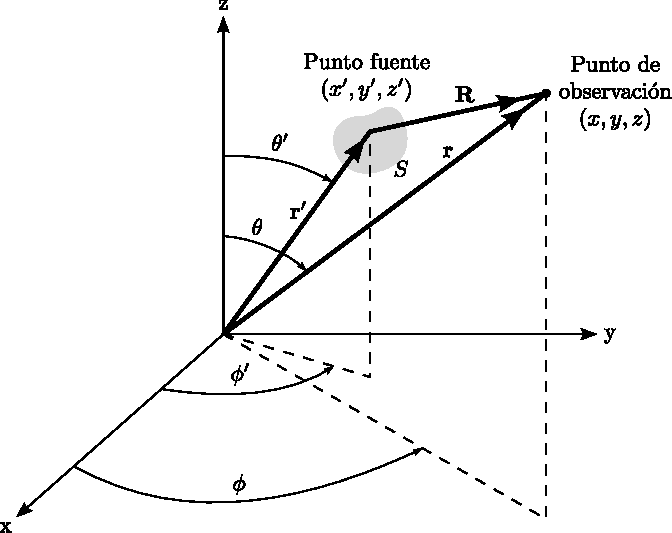
\includegraphics[scale = 0.93]{Figures/Fundamentos/fundamentos_11.pdf}}
\subfigure[Campo lejano.]{
\label{fig_fundamentos:12}
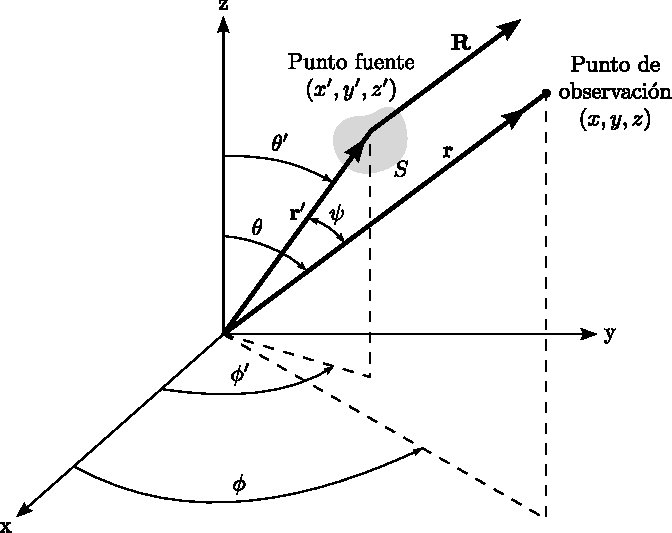
\includegraphics[scale = 0.93]{Figures/Fundamentos/fundamentos_12.pdf}}
\caption{Sistemas de coordenadas para análisis de antenas de abertura.}
\label{grup_fig_fundamentos:5}
\end{figure}
%%%%
Empleando la geometría de la figura \ref{fig_fundamentos:11}, pueden determinarse los campos empleando las expresiones \eqref{ec_fundamentos:41} y \eqref{ec_fundamentos:42}. En la figura \ref{fig_fundamentos:11}, $R$ es la distancia entre cualquier punto fuente sobre la superficie $S$, donde existen $\mathbf{J}_s$ y $\mathbf{M}_s$, y el punto de observación.

Para la mayoría de los problemas, la principal dificultad es la complejidad requerida para resolver las integrales de las expresiones \eqref{ec_fundamentos:41} y \eqref{ec_fundamentos:42}. Sin embargo, para observaciones de campo lejano es posible reducir la complejidad de las integrales. Aplicando el teorema del coseno y desarrollando en serie de Taylor a primer orden, es posible expresar $R$ como:
%%%%
\begin{align}
R = \sqrt{r^2 +{r'}^2 - 2\mathbf{r}'\prodesc\mathbf{r}} \simeq \mathbf{r}'\prodesc\versor{r} = r - r'\cos\psi
\label{ec_fundamentos:43}
\end{align}
%%%%
La simplificación que se emplea es aproximar la amplitud a orden cero y la fase a orden uno, por lo que las aproximaciones formuladas son:
%%%%
\begin{subequations}
\label{grup_ec_fundamentos:2}
\begin{align}
R &\simeq r - r'\cos\psi \mbox{ (para variaciones de fase)}
\label{ec_fundamentos:44}\\
R &\simeq r \mbox{ (para variaciones de amplitud)}
\label{ec_fundamentos:45}
\end{align}
\end{subequations}
%%%%
donde $\psi$ es el ángulo entre los vectores $\mathbf{r}$ y $\mathbf{r}'$. Geométricamente, las aproximaciones de las expresiones \eqref{ec_fundamentos:43} y \eqref{grup_ec_fundamentos:2} asumen que los vectores $\mathbf{R}$ y $\mathbf{r}$ tienen la misma longitud y son paralelos, como se muestra en la figura \ref{fig_fundamentos:12}.

Empleando las aproximaciones \eqref{grup_ec_fundamentos:2}, las expresiones \eqref{ec_fundamentos:41} y \eqref{ec_fundamentos:42} resultan:
%%%%
\begin{align}
\mathbf{A} &= \frac{\mu}{4\pi}\iint\limits_S\mathbf{J}_s\frac{e^{-jkR}}{R}\,ds' \simeq \frac{\mu e^{-jkr}}{4\pi r}\,\mathbf{N}
\label{ec_fundamentos:46}\\
\mathbf{N} &= \iint\limits_S\mathbf{J}_s\,e^{jkr'\cos\psi}ds' = \iint\limits_S\!\left(J_x\versor{x} + J_y\versor{y} + J_z\versor{z}\right)e^{jkr'\cos\psi}ds'
\tag{\ref{ec_fundamentos:46}a}
\label{ec_fundamentos:47}\\
\mathbf{F} &= \frac{\varepsilon}{4\pi}\iint\limits_S\mathbf{M}_s\frac{e^{-jkR}}{R}\,ds' \simeq \frac{\varepsilon e^{-jkr}}{4\pi r}\,\mathbf{L}
\label{ec_fundamentos:48}\\
\mathbf{L} &= \iint\limits_S\mathbf{M}_s\,e^{jkr'\cos\psi}ds' = \iint\limits_S\!\left(M_x\versor{x} + M_y\versor{y} + M_z\versor{z}\right)e^{jkr'\cos\psi}ds'
\tag{\ref{ec_fundamentos:48}a}
\label{ec_fundamentos:49}
\end{align}
%%%%
Usando las expresiones \eqref{ec_fundamentos:46}$-$\eqref{ec_fundamentos:49}, las componentes resultantes de los campos $\mathbf{E}$ y $\mathbf{H}$ son:
%%%%
\begin{subequations}
\label{grup_ec_fundamentos:3}
\begin{align}
E_r &\simeq 0
\label{ec_fundamentos:50}\\
E_{\theta} &\simeq - j\frac{ke^{-jkr}}{4\pi r}\left(L_{\phi} + \eta N_{\theta}\right)
\label{ec_fundamentos:51}\\
E_{\phi} &\simeq j\frac{ke^{-jkr}}{4\pi r}\left(L_{\theta} - \eta N_{\phi}\right)
\label{ec_fundamentos:52}\\
H_r &\simeq 0
\label{ec_fundamentos:53}\\
H_{\theta} &\simeq - \frac{E_{\phi}}{\eta}
\label{ec_fundamentos:54}\\
H_{\phi} &\simeq \frac{E_{\theta}}{\eta}
\label{ec_fundamentos:55}
\end{align}
\end{subequations}
%%%%

%%%%
\subsection{Aberturas rectangulares}
\label{subsec_fundamentos_aber_rect}
%%%%

%%%%
Para el análisis de las aberturas rectangulares, se utiliza el sistema de referencia de la figura \ref{fig_fundamentos:13}.
%%%%
\begin{figure} [H]
\centering 
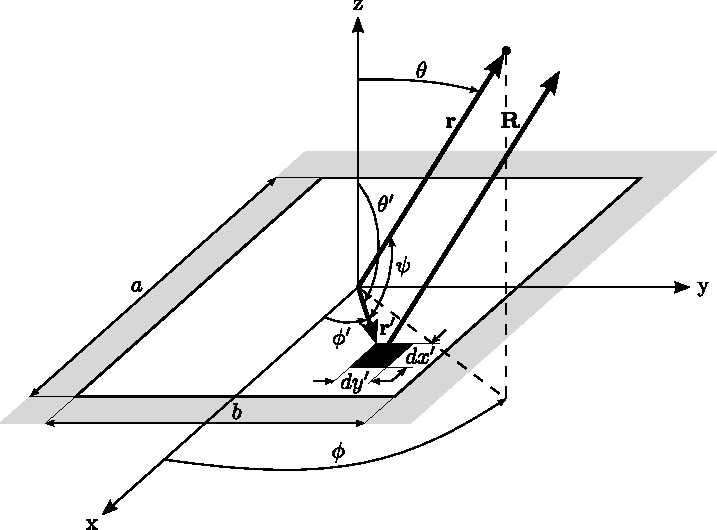
\includegraphics[scale = 1]{Figures/Fundamentos/fundamentos_13.pdf}
\caption{Sistema de referencia para análisis de aberturas rectangulares.}
\label{fig_fundamentos:13}
\end{figure}
%%%%
La expresión de la diferencia de caminos entre el punto fuente y el punto de observación ($r'\cos\psi$) es:
%%%%
\begin{align}
\begin{split}
r'\cos\psi &= \mathbf{r}'\prodesc\versor{r} = \left(x'\versor{x} + y'\versor{y}\right)\prodesc\left(\sen\theta\cos\phi\,\versor{x} + \sen\theta\sen\phi\,\versor{y} + \cos\theta\,\versor{z}\right)\\
&= x'\sen\theta\cos\phi + y'\sen\theta\sen\phi
\end{split}
\label{ec_fundamentos:56}
\end{align}
%%%%
y la del diferencial de área está representada por:
%%%%
\begin{align}
&ds' = dx'dy'
\label{ec_fundamentos:57}
\end{align}
%%%%
Aplicando transformación de coordenadas cartesianas a esféricas a las expresiones \eqref{ec_fundamentos:47} y \eqref{ec_fundamentos:49}, empleando las expresiones \eqref{ec_fundamentos:56} y \eqref{ec_fundamentos:57} y utilizando el sistema de referencia de la figura \ref{fig_fundamentos:13}, puede determinarse $N_{\theta}$, $N_{\phi}$, $L_{\theta}$ y $L_{\phi}$ como:
%%%%
\begin{subequations}
\label{grup_ec_fundamentos:4}
\begin{align}
N_{\theta} &= \!\int_{-b/2}^{\,b/2}\int_{-a/2}^{\,a/2}\!\left(J_x\cos\theta\cos\phi + J_y\cos\theta\sen\phi\right)e^{jkr'\left(x'\sen\theta\cos\phi + y'\sen\theta\sen\phi\right)}dx'dy'
\label{ec_fundamentos:58}\\
N_{\phi} &= \!\int_{-b/2}^{\,b/2}\int_{-a/2}^{\,a/2}\!\left(- J_x\sen\phi + J_y\cos\phi\right)e^{jkr'\left(x'\sen\theta\cos\phi + y'\sen\theta\sen\phi\right)}dx'dy'
\label{ec_fundamentos:59}\\
L_{\theta} &= \!\int_{-b/2}^{\,b/2}\int_{-a/2}^{\,a/2}\!\left(M_x\cos\theta\cos\phi + M_y\cos\theta\sen\phi\right)e^{jkr'\left(x'\sen\theta\cos\phi + y'\sen\theta\sen\phi\right)}dx'dy'
\label{ec_fundamentos:60}\\
L_{\phi} &= \!\int_{-b/2}^{\,b/2}\int_{-a/2}^{\,a/2}\!\left(- M_x\sen\phi + M_y\cos\phi\right)e^{jkr'\left(x'\sen\theta\cos\phi + y'\sen\theta\sen\phi\right)}dx'dy'
\label{ec_fundamentos:61}
\end{align}
\end{subequations}
%%%%

%%%%
\subsection{Aberturas circulares}
\label{sec_fundamentos_aber_circ}
%%%%

%%%%
Para el análisis de las aberturas circulares, se utiliza el sistema de referencia de la figura \ref{fig_fundamentos:14}.
%%%%
\begin{figure} [H]
\centering 
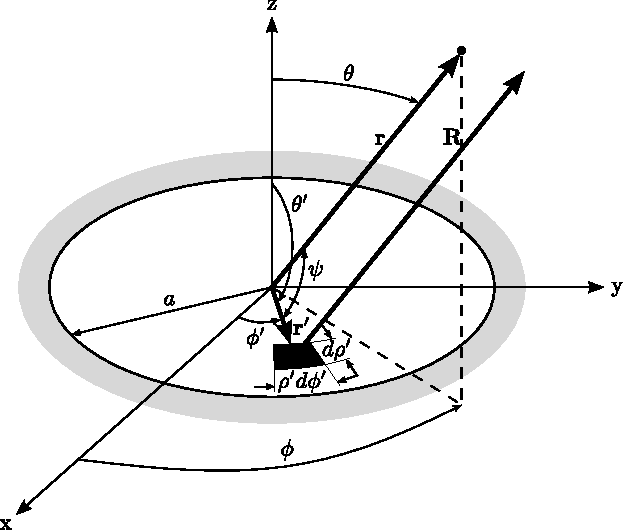
\includegraphics[scale = 1]{Figures/Fundamentos/fundamentos_14.pdf}
\caption{Sistema de referencia para análisis de aberturas circulares.}
\label{fig_fundamentos:14}
\end{figure}
%%%%
Para analizar las aberturas circulares, es conveniente expresar las densidades de corriente $\mathbf{J}_s$ y $\mathbf{M}_s$ en coordenadas cilíndricas. La transformación entre componentes cartesianas y cilíndricas de $\mathbf{J}_s$ está dada por:
%%%% 
\begin{align}
\begin{bmatrix}
J_x\\
J_y\\
J_z
\end{bmatrix}
=
\begin{bmatrix}
\cos\phi ' & -\sen\phi ' & 0\\
\sen\phi ' & \cos\phi ' & 0\\
0 & 0 & 1
\end{bmatrix}
\begin{bmatrix}
J_{\rho}\\
J_{\phi}\\
J_z
\end{bmatrix}
\label{ec_fundamentos:62}
\end{align}
%%%%
Se realiza una transformación similar para las componentes de $\mathbf{M}_s$. Las coordenadas cartesianas y cilíndricas están relacionadas por:
%%%%
\begin{subequations}
\label{grup_ec_fundamentos:5}
\begin{align}
x' &= \rho '\cos\phi '
\label{ec_fundamentos:63}\\
y' &= \rho '\sen\phi '
\label{ec_fundamentos:64}\\
z' &= z'
\label{ec_fundamentos:65}
\end{align}
\end{subequations}
%%%%
Empleando las expresiones \eqref{grup_ec_fundamentos:5} se determina la diferencia de caminos entre el punto fuente y el punto de observación, que queda expresada como:
%%%%
\begin{align}
&r'\cos\psi = x'\sen\theta\cos\phi + y'\sen\theta\sen\phi = \rho '\sen\theta\cos\left(\phi - \phi '\right)
\label{ec_fundamentos:66}
\end{align}
%%%%
mientras que la expresión del diferencial de área está representada por:
%%%%
\begin{align}
&ds' = dx'dy' = \rho 'd\rho 'd\phi '
\label{ec_fundamentos:67}
\end{align}
%%%%
Aplicando transformación de coordenadas cartesianas a esféricas a las expresiones \eqref{ec_fundamentos:47} y \eqref{ec_fundamentos:49}, empleando las expresiones \eqref{ec_fundamentos:66} y \eqref{ec_fundamentos:67} y utilizando el sistema de referencia de la figura \ref{fig_fundamentos:14}, puede determinarse $N_{\theta}$, $N_{\phi}$, $L_{\theta}$ y $L_{\phi}$ como:
%%%%
\begin{subequations}
\label{grup_ec_fundamentos:6}
\begin{flalign}
N_{\theta} &= \!\int_0^{\,a}\int_0^{\,2\pi}\!\rho '\left[J_{\rho}\cos\theta\cos\left(\phi - \phi '\right) + J_{\phi}\cos\theta\sen\left(\phi - \phi '\right)\right]e^{jkr'\rho '\sen\theta\cos\left(\phi - \phi '\right)}d\phi 'd\rho '
\label{ec_fundamentos:68}\\
N_{\phi} &= \!\int_0^{\,a}\int_0^{\,2\pi}\!\rho '\left[- J_{\rho}\sen\left(\phi - \phi '\right) + J_{\phi}\cos\left(\phi - \phi '\right)\right]e^{jkr'\rho '\sen\theta\cos\left(\phi - \phi '\right)}d\phi 'd\rho '
\label{ec_fundamentos:69}\\
L_{\theta} &= \!\int_0^{\,a}\int_0^{\,2\pi}\!\rho '\left[M_{\rho}\cos\theta\cos\left(\phi - \phi '\right) + M_{\phi}\cos\theta\sen\left(\phi - \phi '\right)\right]e^{jkr'\rho '\sen\theta\cos\left(\phi - \phi '\right)}d\phi 'd\rho '
\label{ec_fundamentos:70}\\
L_{\phi} &= \!\int_0^{\,a}\int_0^{\,2\pi}\!\rho '\left[- M_{\rho}\sen\left(\phi - \phi '\right) + M_{\phi}\cos\left(\phi - \phi '\right)\right]e^{jkr'\rho '\sen\theta\cos\left(\phi - \phi '\right)}d\phi 'd\rho '
\label{ec_fundamentos:71}
\end{flalign}
\end{subequations}
%%%%

%%%%
\section{Área efectiva de antenas de abertura}
\label{sec_fundamentos_area_ef_ant_aber}
%%%%

En la sección \ref{subsec_intro_direc}, se definió la directividad máxima $D_0$ de una antena como:
%%%%
\begin{align}
D_0  = 4\pi\frac{U_{max}}{P_{rad}}
\label{ec_fundamentos:72}
\end{align}
%%%%
y en la sección \ref{subsec_intro_area_efec}, se relacionó el área de abertura máxima $A_{em}$ con la directividad máxima de una antena, obteniendo la expresión:
%%%%
\begin{align}
D_0  = \frac{4\pi}{\lambda^2}A_{em}
\label{ec_fundamentos:73}
\end{align}
%%%%
A partir de las expresiones \eqref{ec_fundamentos:72} y \eqref{ec_fundamentos:73}, se deduce que el área efectiva máxima está relacionada con la intensidad de radiación máxima y la potencia radiada por la antena.

Empleando las expresiones \eqref{ec_fundamentos:51} y \eqref{ec_fundamentos:52}, la intensidad de radiación queda expresada como:
%%%%
\begin{align}
U\left(\theta,\phi\right) &= \frac{k^2}{32\pi^2\eta}\left[\vert L_{\phi} + \eta N_{\theta}\vert^2 + \lvert L_{\theta} - \eta N_{\phi}\rvert^2\right]
\label{ec_fundamentos:74}
\end{align}
%%%%
y sabiendo que $k = \dfrac{2\pi}{\lambda}$, la expresión \eqref{ec_fundamentos:74} se reduce a:
%%%%
\begin{align}
U\left(\theta,\phi\right) &= \frac{1}{8\eta\lambda^2}\left[\vert L_{\phi} + \eta N_{\theta}\vert^2 + \lvert L_{\theta} - \eta N_{\phi}\rvert^2\right]
\label{ec_fundamentos:75}
\end{align}
%%%%
Considerando que la abertura es rectangular, el campo eléctrico sobre la abertura $\mathbf{E}_a$ se expresa como:
%%%%
\begin{align}
\mathbf{E}_a &= E_{ax}\,\versor{x} + E_{ay}\,\versor{y} 
\label{ec_fundamentos:76}
\end{align}
%%%%
Los campos sobre la abertura $\mathbf{E}_a$ y $\mathbf{H}_a$ están relacionados entre sí por la expresión \eqref{ec_fundamentos:32}, por lo que las densidades de corriente $\mathbf{J}_s$ y $\mathbf{M}_s$ pueden expresarse en función de las componentes de $\mathbf{E}_a$; las expresiones \eqref{ec_fundamentos:30} y \eqref{ec_fundamentos:31}, entonces, se reducen a:
%%%%
\begin{align}
\mathbf{J}_s &= -\dfrac{E_{ax}}{\eta}\versor{x} - \dfrac{E_{ay}}{\eta}\versor{y} 
\label{ec_fundamentos:77}\\
\mathbf{M}_s &= -E_{ax}\,\versor{y} + E_{ay}\,\versor{x} 
\label{ec_fundamentos:78}
\end{align}
%%%%
Considerando que la intensidad de radiación máxima se produce para $\theta = 0$, las expresiones \eqref{grup_ec_fundamentos:4} se reducen a:
%%%%
\begin{subequations}
\label{grup_ec_fundamentos:7}
\begin{align}
N_{\theta} &= \!\iint\limits_S\!\left(-\dfrac{E_{ax}}{\eta}\cos\phi - \dfrac{E_{ay}}{\eta}\sen\phi\right)ds'
\label{ec_fundamentos:79}\\
N_{\phi} &= \!\iint\limits_S\!\left(\dfrac{E_{ax}}{\eta}\sen\phi - \dfrac{E_{ay}}{\eta}\cos\phi\right)ds'
\label{ec_fundamentos:80}\\
L_{\theta} &= \!\iint\limits_S\!\left(E_{ay}\cos\phi - E_{ax}\sen\phi\right)ds'
\label{ec_fundamentos:81}\\
L_{\phi} &= \!\iint\limits_S\!\left(-E_{ay}\sen\phi - E_{ax}\cos\phi\right)ds'
\label{ec_fundamentos:82}
\end{align}
\end{subequations}
%%%%
y combinando las expresiones \eqref{grup_ec_fundamentos:7}, se obtiene:
%%%%
\begin{subequations}
\label{grup_ec_fundamentos:8}
\begin{align}
L_{\phi} + \eta N_{\theta} &= -2\!\iint\limits_S\!\left(E_{ax}\cos\phi + E_{ay}\sen\phi\right)ds'
\label{ec_fundamentos:83}\\
L_{\theta} - \eta N_{\phi} &= -2\!\iint\limits_S\!\left(E_{ax}\sen\phi - E_{ay}\cos\phi\right)ds'
\label{ec_fundamentos:84}
\end{align}
\end{subequations}
%%%%
A partir de las expresiones \eqref{grup_ec_fundamentos:8}, se deduce:
%%%%
\begin{subequations}
\label{grup_ec_fundamentos:9}
\begin{align}
\begin{split}
\lvert L_{\phi} + \eta N_{\theta}\rvert^2 &= 4\left(\cos^2\phi\left|\iint\limits_S\! E_{ax}\, ds'\right|^2 + \sen^2\phi\left|\iint\limits_S\! E_{ay}\, ds'\right|^2\right.\\
&\left.+ 2\sen\phi\cos\phi\iint\limits_S\! E_{ax}\, ds'\iint\limits_S\! E_{ay}\, ds'\right)
\end{split}
\label{ec_fundamentos:85}\\
\begin{split}
\lvert L_{\theta} - \eta N_{\phi}\rvert^2 &= 4\left(\sen^2\phi\left|\iint\limits_S\! E_{ax}\, ds'\right|^2 + \cos^2\phi\left|\iint\limits_S\! E_{ay}\, ds'\right|^2\right.\\
&\left.- 2\sen\phi\cos\phi\iint\limits_S\! E_{ax}\, ds'\iint\limits_S\! E_{ay}\, ds'\right)
\end{split}
\label{ec_fundamentos:86}
\end{align}
\end{subequations}
%%%%
y sumando las expresiones \eqref{ec_fundamentos:85} y \eqref{ec_fundamentos:86}, se obtiene:
%%%%
\begin{align}
\lvert L_{\phi} + \eta N_{\theta}\rvert^2 + \lvert L_{\theta} - \eta N_{\phi}\rvert^2 &= 4\left(\,\left|\iint\limits_S\! E_{ax}\, ds'\right|^2 + \left|\iint\limits_S\! E_{ay}\, ds'\right|^2\,\right) = 4\left|\iint\limits_S\mathbf{E}_a\, ds'\right|^2
\label{ec_fundamentos:87}
\end{align}
%%%%
La intensidad de radiación máxima queda expresada como:
%%%%
\begin{align}
U_{max} &= \dfrac{1}{2\eta\lambda^2}\left|\iint\limits_S\mathbf{E}_a\, ds'\right|^2
\label{ec_fundamentos:88}
\end{align}
%%%%
En la sección \ref{subsec_intro_pot_med_rad}, se definió la potencia radiada por una antena $P_{rad}$ como:
%%%%
\begin{align}
P_{rad} = \!\iint\limits_S\mathbf{W}_{av}\prodesc\versor{n}\,ds' = \dfrac{1}{2}\!\iint\limits_S\Re\left(\mathbf{E}\prodvec\mathbf{H}^*\right)\prodesc\versor{n}\,ds'
\label{ec_fundamentos:89}
\end{align}
%%%%
Reemplazando $\mathbf{E}$ por $\mathbf{E}_a$ y $\mathbf{H}$ por $\mathbf{H}_a$, la expresión \eqref{ec_fundamentos:89} se reduce a:
%%%%
\begin{align}
P_{rad} = \dfrac{1}{2\eta}\!\iint\limits_S\left(\lvert E_{ax}\rvert^2 + \lvert E_{ay}\rvert^2\right)ds' = \dfrac{1}{2\eta}\!\iint\limits_S\lvert \mathbf{E}_a\rvert^2 ds'
\label{ec_fundamentos:90}
\end{align}
%%%%
Incluyendo las expresiones \eqref{ec_fundamentos:88} y \eqref{ec_fundamentos:90} en la expresión \eqref{ec_fundamentos:72}, la directividad máxima queda expresada como:
%%%%
\begin{align}
D_0  = 4\pi\dfrac{\dfrac{1}{2\eta\lambda^2}\left|\displaystyle\iint\limits_S\mathbf{E}_a\, ds'\right|^2}{\dfrac{1}{2\eta}\!\displaystyle\iint\limits_S\lvert \mathbf{E}_a\rvert^2 ds'}  = \dfrac{4\pi}{\lambda^2}\dfrac{\left|\displaystyle\iint\limits_S\mathbf{E}_a\, ds'\right|^2}{\displaystyle\iint\limits_S\lvert \mathbf{E}_a\rvert^2 ds'}
\label{ec_fundamentos:91}
\end{align}
%%%%
A partir de  la expresión \eqref{ec_fundamentos:73}, se deduce que:
%%%%
\begin{align}
A_{em}  = \dfrac{\left|\displaystyle\iint\limits_S\mathbf{E}_a\, ds'\right|^2}{\displaystyle\iint\limits_S\lvert \mathbf{E}_a\rvert^2 ds'}
\label{ec_fundamentos:92}
\end{align}
%%%%
Empleando la expresión \eqref{ec_intro:54} se determina la eficiencia de abertura, que resulta:
%%%%
\begin{align}
\varepsilon_{ap}  = \dfrac{\left|\displaystyle\iint\limits_S\mathbf{E}_a\, ds'\right|^2}{A_p\!\displaystyle\iint\limits_S\lvert\mathbf{E}_a\rvert^2 ds'}
\label{ec_fundamentos:93}
\end{align}
%%%%
Si bien se partió del supuesto de que la abertura era rectangular para deducir la expresión \eqref{ec_fundamentos:93}, la misma es válida también para aberturas circulares.

Dado que la integral del numerador de la expresión \eqref{ec_fundamentos:93} depende tanto de la magnitud como de la fase de $\mathbf{E}_a$, se separan ambos efectos \cite{Orfanidis} definiendo:
%%%%
\begin{subequations}
\label{grup_ec_fundamentos:10}
\begin{align}
\varepsilon_t  = \dfrac{\left|\displaystyle\iint\limits_S\lvert \mathbf{E}_a\rvert\, ds'\right|^2}{A_p\!\displaystyle\iint\limits_S\lvert \mathbf{E}_a\rvert^2 ds'}
\label{ec_fundamentos:94}\\
\varepsilon_p  = \dfrac{\left|\displaystyle\iint\limits_S\mathbf{E}_a\, ds'\right|^2}{\left|\displaystyle\iint\limits_S\lvert \mathbf{E}_a\rvert\, ds'\right|^2}
\label{ec_fundamentos:95}
\end{align}
\end{subequations}
%%%%
donde:
%%%%
\begin{align*}
\varepsilon_t &= \text{Eficiencia de iluminación.}\\
\varepsilon_p &= \text{Eficiencia de fase.}
\end{align*}
%%%%
y entonces la eficiencia de abertura queda expresada como:
%%%%
\begin{align}
\varepsilon_{ap}  = \varepsilon_t\varepsilon_p
\label{ec_fundamentos:96}
\end{align}
%%%%
